% $Id: SECTIONS.tex 10532 2010-03-16 15:57:20Z alexandra $
% Local Variables:
% ispell-check-comments: nil
% Local IspellDict: american
% End:
% --------------------------------------------------------
% User documentation
% copyright by BREDEX GmbH 2004
% --------------------------------------------------------

% This file includes all section for ,,Getting Started''
% ---------------------------------------------------
\jb{} is a tool for the automated testing of Graphical User Interfaces (GUI's) written with Java (Swing, SWT/RCP, GEF) and HTML. The focus of the tool is on testing an application's business logic (workflows, use cases)  from the user perspective (functional, black-box, acceptance testing).
 
\jb{} is a keyword-driven tool. Tests are automated by dragging and dropping pre-defined modules (or \gdcases{}, or keywords) to make sequences of actions for your application. Each \jb{} \gdproject{}  contains one or more libraries of these pre-defined modules for you to use. Test automation with these keywords is hierarchical -- using the libraries, you can create modules of your own and reuse them to make more complex tests and so on. 

Using the keyword-driven approach has various advantages, which are detailed in the next section \bxpref{JBApproach}. 

\section{\jb{} compared to other testing approaches}
% $Id: approaches.tex 7776 2009-01-30 17:08:26Z alexandra $
% Local Variables:
% ispell-check-comments: nil
% Local IspellDict: american
% End:
% --------------------------------------------------------
% User documentation
% copyright by BREDEX GmbH 2004
% --------------------------------------------------------

Testing is critical to the success of software projects. It is especially important to acceptance test software which is designed for end users.

There are various ways to go about performing acceptance testing, each with their advantages and disadvantages. 

\subsection{Manual Tests}

Manual testing, although thorough, cannot keep up with the pace of development. It is impossible to carry out complete continuous integration and regression tests manually. 


\subsection{Programmed Tests}

Writing tests in some kind of scripting language is certainly powerful, but it puts a strain on the resources of a team, because the test code itself becomes a project in its own right and also needs to be checked and maintained. The extra costs added by programming GUI tests can be considerable. 

Tests written in code also have the problem that they no longer view the software as a black box and may miss important aspects relating to the acceptance. In addition, automation experts (experienced software developers) become the only people who can write or maintain tests. It is generally inadvisable to test your own work, but this is what can happen if testing remains solely in the realm of the developers. Writing tests without coding from the black box perspective not only allows test experts to automate tests (and therefore brings the test perspective to the forefront), but also puts developers in the shoes of the users, which helps to focus and improve the test.  


\subsection{Recorded Tests}

Possibly the most popular approach to automated functional testing is macro recording, that is, recording a user's actions for later playback.
The appeal of this approach is the apparently quick success that can be seen: a test script can be quickly recorded and played back, giving the impression that automated testing is nothing more than recording a manual test. 

However, this approach fails to meet the needs of large or long-term software projects for the following reasons:

\begin{itemize}
\item Test specification begins very late in the development cycle,
 as recording can only begin once the software is available. 
\item Since only the user action is recorded, checkpoints for verification
of test results have to be inserted manually.
\item Recorded tests can only test parts of the application which already work. \item There is also the danger that the implementation of the application will be tested, instead of the requirements. 
\item Recorded scripts are often very large and not particularly 
well-structured. Making changes at a later point is therefore 
difficult and requires programming skills, which further increases costs.  
\item Code generated by recording generally doesn't conform to
 common software quality attributes such as reliability, stability, 
portability, maintainability, and usability.
\end{itemize}

In essence, a recorded script is not an automated test. It must be refactored to remove errors and redundancies, to make its component parts modular and reusable and to insert the intelligence of the manual tester to make the test robust. Once all this has been done, there is probably very little of the original recording left, and a great deal of development work has been done to refactor the script.  


\subsection{The \jb{} approach}
\label{JBApproach}
\jb{} makes lets you automate tests which follow the best practices known from software development (readability, modularity and reusability to ensure maintainability), but without any programming effort. 


This gives the following advantages: 

\subsection{Early test creation}

\jb{} tests are created before the \gdaut{} is available. This is a radical advantage over capture-replay tools, which force testers to wait until an application is ready to begin with testing. The specification of modular, flexible GUI tests begins early (even as early as at the requirements stage) and continues alongside software development.\\ 
The benefit of this is that every version of an \gdaut{} can be tested as soon as it becomes available. Testing keeps up with development, so you waste no time in your test process. Earlier testing lets you find issues when they are cheaper and easier to fix and encourages collaboration and communication within the team.

\subsection{Code-free automation}

Tests are automated completely from the user perspective and require no programming effort. \\

This means that those who understand the user perspective best are able to fully automate tests. There is no need to wait for input (e.g. programmatic creation of test modules) from other team members to automate a test. If developers are writing tests, the black box perspective encourages them to think like a user would when faced with the software. Code-free tests also have the advantage that they are readable by the whole team and also by users or customers. 


\subsection{Manual tester intelligence}

The wide range of keywords available in \jb{} include high-level actions which can be meaningfully used by testers. There is also a wide range of check and synchronization actions to incorporate the necessary robustness into a test. 


\clearpage

\section{How to read this manual}
The amount of keywords you have in a \app{} test and the amount of components your test deals with can grow very quickly. For this reason, it is important to think about structuring the \gdtestcasebrowser{} and the \gdomeditor{} to make finding \gdcases{} and component names easier. 


\subsection{Configuring task repositories in your workspace}
\label{TasksALMConfigureWorkspace}
Each repository you want to work with in your \ite{} must be configured in the workspace you are using. 

\begin{enumerate}
\item Select:\\ \bxmenu{Window}{Show View}{Other}\\ from the menu.
\item In the \bxname{Mylyn} section, select \bxname{Task Repositories} and click \bxcaption{OK}. The \bxname{Task Repositories} View will appear. The Bugzilla Repositories for \gd{} and \jb{} are pre-configured.
\item In the \bxname{Task Repositories} View, right click and select \bxname{Add Task Repository} from the context menu.
\item In the dialog that appears, you will see the pre-defined task repositories for the \ite{}. You can select one of these or choose to install a different connector. Depending on the connector you want to use, you may require additional software from Tasktop, or the connector may incur license fees.
\item Once you have selected your connector, click \bxcaption{Next}.
\item On the following page, you will need to configure the task repository. Please refer to the Mylyn documentation for information on repository configuration. 
\item Click \bxcaption{Finish} once the repository is configured.
\item To be able to see tasks in this repository, select: \\ \bxmenu{Window}{Show View}{Other}\\ from the menu. 
\item In the \bxname{Mylyn} section, select \bxname{Task List} and click \bxcaption{OK}. The \bxname{Task List} View will appear.
\end{enumerate}

You will now be able to see items in this repository, open them in the \ite{}, add queries for your workspace and work on tasks from this repository. 
You will also be able to select this repository in the \gdproject{} properties as the repository for your \gdproject{} \bxpref{TasksALMConfigureProject}. 


\subsection{Working on tasks in the \ite{}: contexts}
Once you have configured a task repository for your workspace \bxpref{TasksALMConfigureWorkspace}, you can work on tasks from that repository. 

\subsubsection{Opening and editing tasks in the \ite{}}
\begin{itemize}
\item To be able to see tasks in a repository, select: \\ \bxmenu{Window}{Show View}{Other}\\ from the menu. 
\item In the \bxname{Mylyn} section, select \bxname{Task List} and click \bxcaption{OK}. The \bxname{Task List} View will appear.
\item Double-click on a task to open this task in the editor area.
\item Once a task is open, you can work on it as you would in an external system -- add comments, change status etc.
\end{itemize}

\subsubsection{Working on tasks in the \ite{}}
\label{TasksActivateTask}
Mylyn supports context- or task-based working. When you work on a task, you only see items relevant to that task, so that coming back to the task later involves less context-switching. 
\begin{itemize}
\item Mylyn supports context-based working. You can work on existing tasks in a configured repository, or you can create tasks to work on.
\item To work on a task, you must \bxname{activate} it. To activate a task, select the task in the \bxname{Task List} and select:\\ \bxmenu{Activate}{}{}\\
from the context-sensitive menu. 
\item When you activate a task for the first time, the browsers and editors will seem very empty. This is because nothing is yet a part of the context for this task.
\item You can navigate through the browsers by pressing \bxkey{Alt+Click} to expand each level, or you can press the \bxname{Focus on task} button in the browsers to show the whole tree (not focusing on the task), or just the items in the current context (focusing on the task). 
\item Items are automatically added to your context when you select them in a browser, when you open them in an editor, or when you perform other actions that cause them to be made relevant (e.g. \gdcase{} creation, showing a \gdcase{} specification etc.). Items that are used particularly frequently are marked as \bxname{landmarks} and shown in bold. 
\item You can manually alter which items are in your context using the context-sensitive menu for a specific item. You can manually make items landmarks, or remove them from the context. 
\item The context that is created for you will be re-created when you reactivate the task at a later point. 
\end{itemize}



\subsection{Creating tasks in external repositories from test result reports}
\gdhelpid{testResultViewContextId}{Test Results View}
 You can create a new task with pre-filled information directly from an open test result report in the \gdtestresultview{}. This is useful if a test has failed and you want to create e.g. an issue in your bug-tracking system for the failure. 
\begin{enumerate}
\item In an open test result report, select the node that best describes the test failure (e.g. a \gdcase{} or \gdstep{} that has failed, or the whole \gdsuite{}, then right-click and select:\\
\bxmenu{Create a Mylyn Task}{}{}\\
from the context-sensitive menu.
\item  In the dialog that appears, select a repository in which to create the task. A \bxname{local} repository is available by default, but you can also add connections to Bugzilla and Trac repositories by clicking \bxcaption{Add Task Repository} in the New Task Dialog. Connectors to other repositories can also be added. See the Mylyn documentation for more details on adding repositories.
\item Click \bxcaption{Finish} once you have selected your repository. 
\item The editor for a new task will appear. It is pre-filled with information relevant to the node that you selected. Edit the task to make it descriptive enough for a bug report and save the editor. 
\item Once you have created a task, you can activate it to start saving your context for this task. See the later section \bxpref{TasksActivateTask} for details.
\end{enumerate}


\subsection{Configuring a task repository for your \gdproject{}}
\label{TasksALMConfigureProject}
Once you have configured one or more repositories for your workspace \bxpref{}, you can select one of these to be the test-relevant repository for your \gdproject{}. 

This will let you:
\begin{itemize}
\item Add a task ID from this repository to \gdcases{}, \gdsuites{}, and \gdjobs{} in the \gdproject{} to signify that this item is the test for this task \bxpref{TasksALMAddTask}.
\item Automatically report test results to the task defined when a test runs.
\item View the test results for the relevant item in the dashboard as a link from the task repository.
\end{itemize}

To configure a task repository for your \gdproject{}:

\begin{enumerate}
\item In the \gdproject{} Properties, select \bxname{Mylyn ALM} from the tree on the left \bxfigref{TasksALMProjectProperties}.
\item In the page that appears, you can select a repository from the combo-box.
\item You can then choose whether to only report failed tests, only report successful tests, or both.
\item Enter the URL of the \dash{} that is configured to use the correct \gddb{} for your test results. This is the \dash{} that will be opened when you click on a test result link from the task repository.
\end{enumerate}

\begin{figure}[h]
\begin{center}
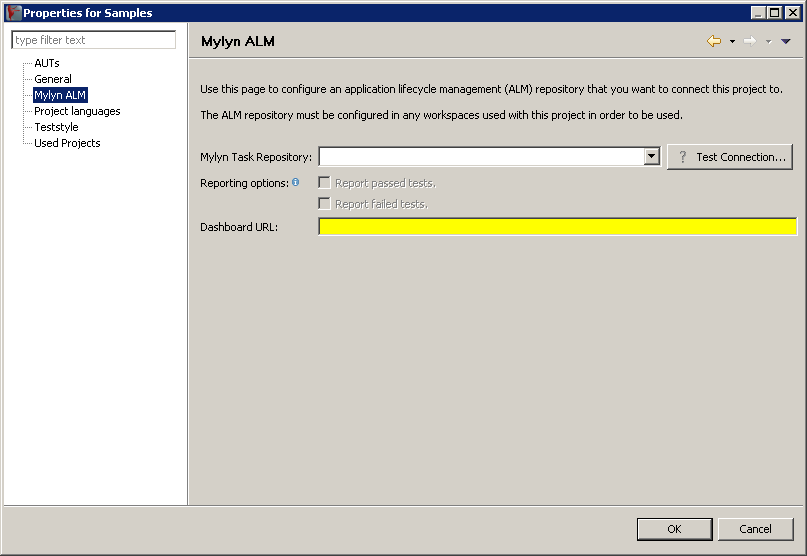
\includegraphics[width=12.5cm]{Tasks/ALM/PS/almproperties}
\caption{ALM Settings}
\label{TasksALMProjectProperties}
\end{center}
\end{figure}


\subsection{Adding task IDs to \gdjobs{}, \gdsuites{} and \gdcases{}}
\label{TasksALMAddTask}
You can add a task ID to \gdcases{}, \gdsuites{} and \gdjobs{} in your \gdproject{}. 

The task ID should be a valid ID in the repository that you have specified as the repository for this \gdproject{} \bxpref{TasksALMConfigureProject}. Adding the task ID to an item in your \gdproject{} means that this item is the relevant test for that task in your repository. When you activate the option, any test results for this item will be added as a comment to the task in the repository. The comment will include a link to the dashboard, in which the test result report can be viewed.

To add a task ID to a \gdcase{}, \gdsuite{} or \gdjob{}:
\begin{enumerate}
\item Open the item in the editor by double-clicking it.
\item In the \gdpropview{}, in the cell for \bxname{Task ID}, enter the task ID from the external repository. You can only enter task IDs at the place of specification -- you cannot overwrite them when you reuse the item.
\item Save the editor. 
\item When you have added a task ID to a node, you can open the task for this node from the browser by selecting:\\
\bxmenu{Open with}{Mylyn Task Editor}{}
\end{enumerate}

\bxtipp{You should ensure that you add task IDs to the right node-level to provide you with the relevant amount of information for the tasks in your repository. This will usually be at the level of Use Cases within a \gdsuite{}. }



\clearpage




